\documentclass[12pt, oneside]{book}

\usepackage{import}
\usepackage{../Packages/baupreamble}


\begin{document}
\chapter{Results and Discussion}

%%=================================================
%%++++++++++++ Start writing here +++++++++++++++++
%%=================================================

\section{My first results}
	This is a random paragraph with a figure (\Mref{figR1}). \lipsum*[3-4]
	
	\begin{figure}[]
		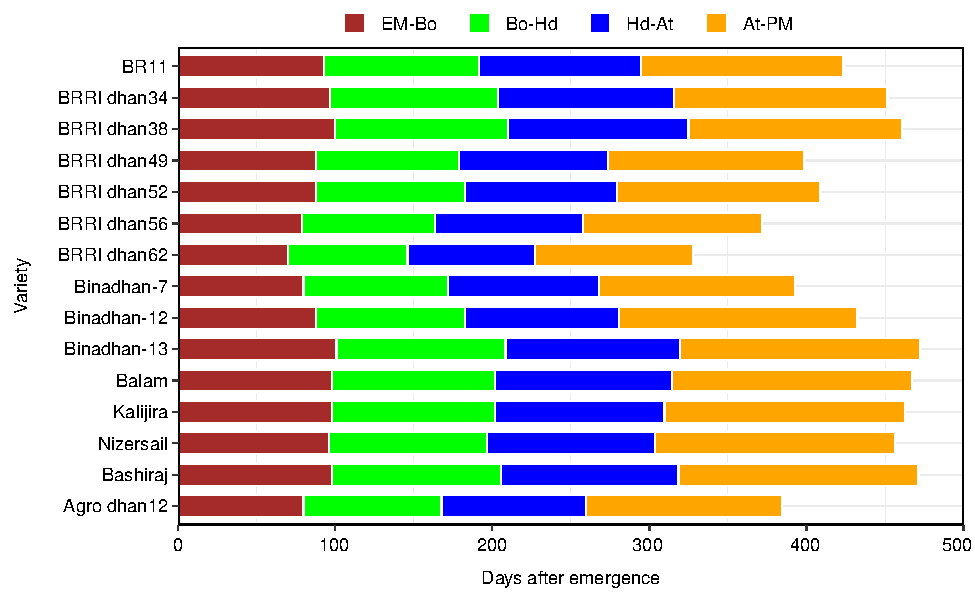
\includegraphics[width=\textwidth]{figures/figR1.pdf}
		\caption{In large projects, such as books, keeping parts of your document in several tex files makes the task of correcting errors and making further changes easier}
		\label{figR1}
	\end{figure}
	
	\subsection{Some results sub-section}
	\lipsum*[1-2]
	\subsubsection{A subsubsection}
			\lipsum*[4]
	\subsubsection{Another subsubsection}
			\lipsum*[5]
	
	\subsection{Another results sub-section}
	This is a paragraph with a table reference (\Mref{tableR1}~ and \Mref{tableA1}). \lipsum*[6]. \textcite{Moradi2020} stated that there are some interesting results which I will not disclose!
	
	% Please add the following required packages to your document preamble:
% \usepackage{multirow}
\begin{table*}[]
	\caption{Climatic data of the study site during the experiment \label{tableR1}}
\begin{tabular*}{\textwidth}{l@{\extracolsep{\fill}}llll}
\toprule
\multirow{2}{*}{Date} & \multirow{2}{*}{RH\%} & \multicolumn{2}{c}{Temperature ($\celsius$)} & \multirow{2}{*}{Rainfall (mm)} \\ \cmidrule(){3-4} 
                      &                       & Max. temp.              & Min. temp.             &                                \\ \midrule
2017-Dec              & 94.85                 & 25.49                 & 11.62                & 0                              \\
2018-Jan              & 95.5                  & 20.92                 & 8.52                 & 0.6                            \\
2018-Feb              & 86.84                 & 26.4                  & 12.64                & 0                              \\
2018-Mar              & 70.61                 & 32.62                 & 18                   & 26                             \\
2018-April            & 68.07                 & 34.49                 & 22.27                & 35.1                           \\
2018-May              & 71.21                 & 34.38                 & 24.32                & 14.5                           \\ \hline
\end{tabular*}
\end{table*}
	
\section{My Second results}

This is a paragraph which contains a reference to a plate (\Mref{plateR1}~and \Mref{figA2}). \lipsum*[11-17]. Now I am going add some citations of previous works \parencite{Devi2012,Karlsson2021,BBS2022}.

\begin{plate}[]
\centering
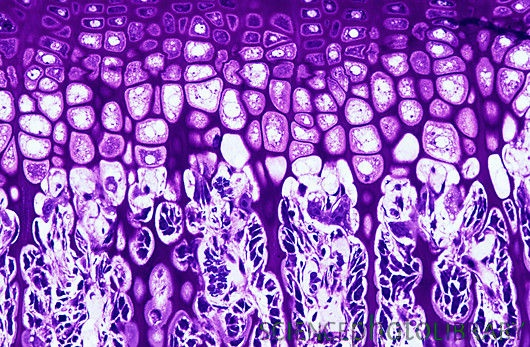
\includegraphics[width=0.5\textwidth]{figures/plateR1}
\caption{Bone growth. Light micrograph of actively growing cells in the growth plate of a long bone}
\label{plateR1}
\end{plate}


\lipsum*[2-4]


%%=================================================
%%=================================================	
\end{document}